\chapter{Results}
\section{Six DOF Stewart Platform}
As earlier mentioned, the Stewart platform has already been designed and fabricated and our part in this work was to do an evaluation of the same to verify its mechanical feasibility. As such, the various parts of the platform were obtained and assembled. For further analysis, a 3D model of the same platform was done using Autodesk Inventor.

The assembled Stewart platform is as shown in figure \ref{fig}. Figure \ref{fig1} shows the Stewart platform configuration setup with the Wind tunnel's test section.
\begin{center}
	\begin{figure}[H]
	\centering
	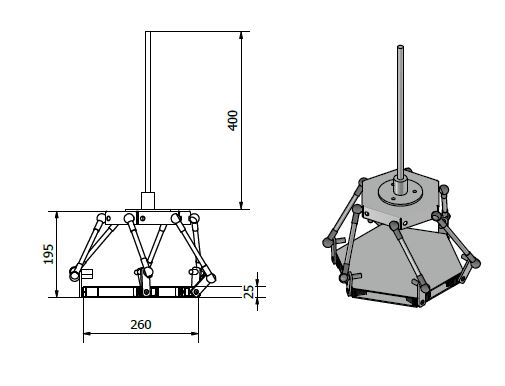
\includegraphics[width=0.8\linewidth]{Figures/Assembly}
	\caption[Assembled Platform]{Assembly of Stewart Platform}
	\label{fig}
	\end{figure}
\end{center}
\begin{center}
	\begin{figure}[H]
	\centering
	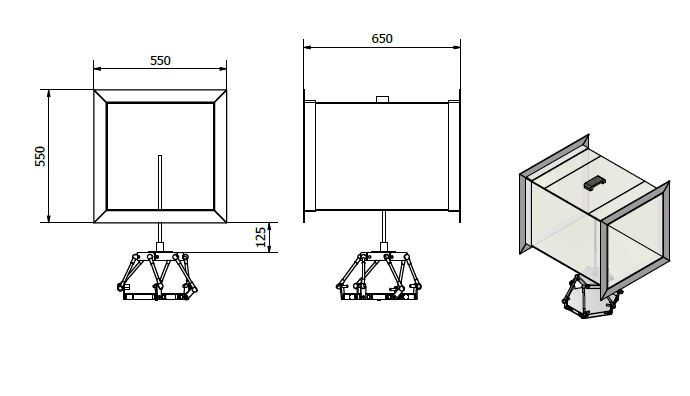
\includegraphics[width=0.8\linewidth]{Figures/Test-section}
	\caption[Model placement in Test Section]{Stewart platform and Test section configuration}
	\label{fig1}
	\end{figure}
\end{center}
Assembling the Stewart platform legs as shown in \ref{fig} makes it easier to achieve the six degrees of freedom as opposed to having two legs attached on the same flange as in figure \ref{fig2}.
\begin{center}
\begin{figure}[H]
\centering
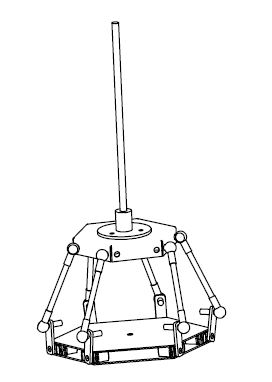
\includegraphics[width=0.3\linewidth]{Figures/assembly2}
\caption[Stewart platform assembly]{Stewart platform alternative assembly}
\label{fig2}
\end{figure}
\end{center}
\subsection{Stability}
The base of the Stewart platform has a bigger diameter (300mm) than that of the moving platform (200mm) hence the center of gravity will always fall within the base during operation. The Stewart platform is therefore stable.
\subsection{Mechanical Feasibility}
Based on the base and platform diameters, distance between the base and platform (i.e. height), an angle of attack of 0.25, and side slip angle of 0.16667, the quality index ($\lambda$) of the Stewart platform was found to be 0.86. This presents a design with few singularities. It is therefore mechanically feasible.
\subsection{Weight}
3D models of the Stewart platform were modeled on Autodesk Inventor using the three materials described earlier. Use of aluminum was verified to offer the most light-weight design.
\begin{table}[H]
\caption{Weight Comparisons}
\end{table}
\begin{center}
\begin{tabular}{|l|l|}
\hline
\textbf{Material} & \textbf{Mass(Kg)}\\
\hline
Aluminium & 2.8\\
\hline
Mild Steel & 4.6\\
\hline
Stainless steel & 5.0 \\
\hline
\end{tabular}
\end{center}
\subsection{Finite Element Analysis on Stewart Platform}
Finite Element Analysis was done on FEA environment in Autodesk inventor. A static analysis test was performed and the following results were obtained:
\begin{table}[H]
\caption{FEA Results}
\end{table}
\begin{center}
\begin{tabular}{|l|l|l|}
\hline
\textbf{Name} & \textbf{Minimum} & \textbf{Maximum}\\
\hline
Von Mise's & 0 MPa & 63.19 MPa\\
\hline
Displacement & 0 mm & 23.74 mm\\
\hline
Safety Factor & 10.3426 ul & 15 ul\\
\hline
Equivalent Strain & 0 ul & 0.052 ul\\
\hline
\end{tabular}
\end{center}
Von Mise's stress does not exceed the Yield Stress of Aluminum (275 MPa) hence the platform will not yield under this applied load.

Application of loads on the platform translates to induced strain in the Stewart platform legs. Such strains are shown in figure \ref{eq}.
\begin{center}
	\begin{figure}[H]
	\centering
	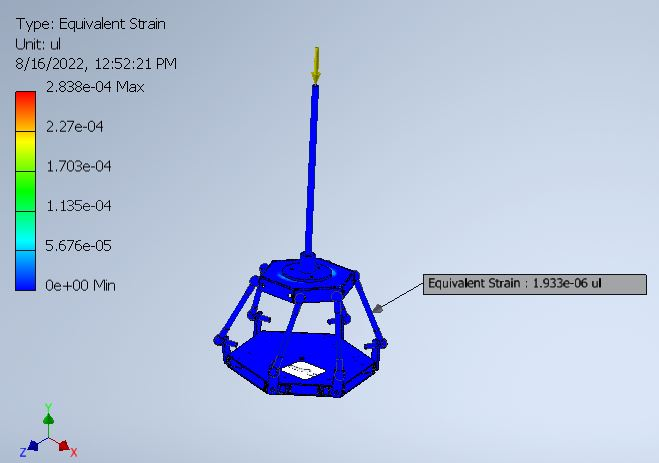
\includegraphics[width=0.6\linewidth]{Figures/Equivalent}
	\caption[Equivalent strain]{Strain induced on each of the legs}
	\label{eq}
	\end{figure}
\end{center}
These strains are small thus they will need amplification in order provide substantial input for the strain gauges used for force measurements. 
\subsection{Stewart Platform Simulation}
Stewart Platform simulation was done on MatLab using the Inverse kinematic equations. Different servo angles for different platform movements can be obtained from the simulation. The angles for yaw, pitch and roll could be adjusted during simulations to predict the maximum allowable angle values. Value of displacement in the x-, y- and z-directions could also be adjusted enabling us to predict the maximum allowable displacement in the respective directions.
\begin{center}
	\begin{figure}[H]
	\centering
	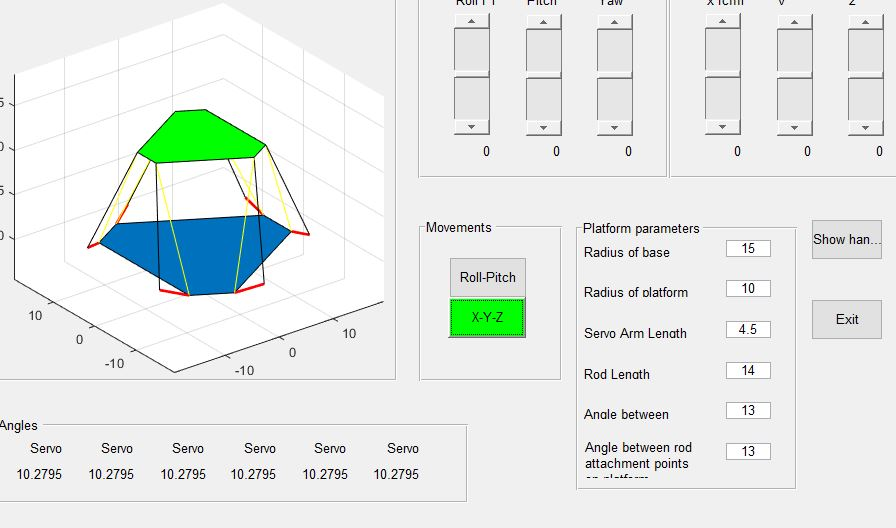
\includegraphics[width=0.75\linewidth]{Figures/Matlab}
	\caption[Linear displacements]{Matlab simulation for x-y-z movements}
	\end{figure}
\end{center}
\begin{center}
	\begin{figure}[H]
	\centering
	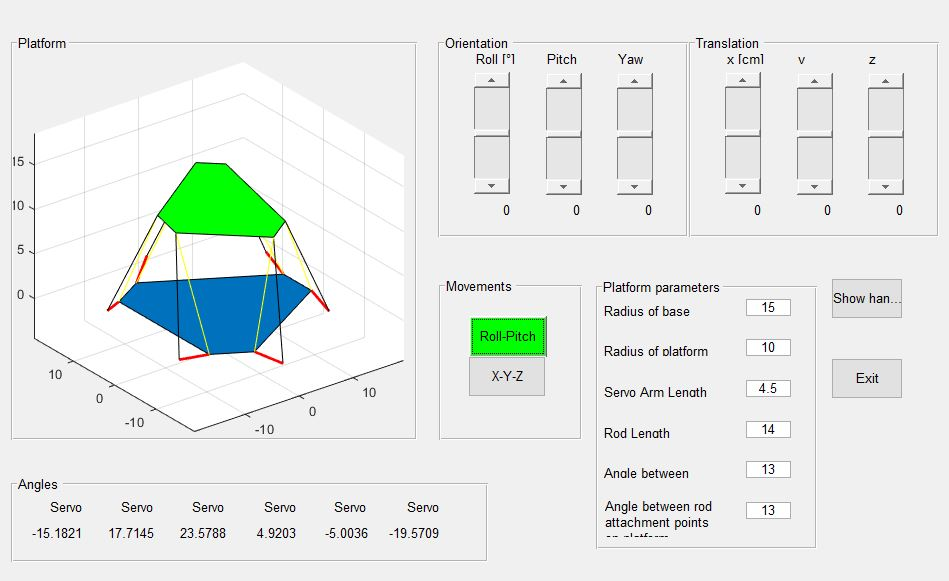
\includegraphics[width=0.75\linewidth]{Figures/Matlab2}
	\caption[Angular displacements]{Matlab simulation for yaw,pitch and roll movements}
	\end{figure}
\end{center}


\section{Human Machine Interface}
The user interface of the platform was programmed using golang and this resulted in the view below with the use of sliders for platform positioning and buttons to set model orientations and start data collection.
\begin{center}
	\begin{figure}[H]
	\centering
	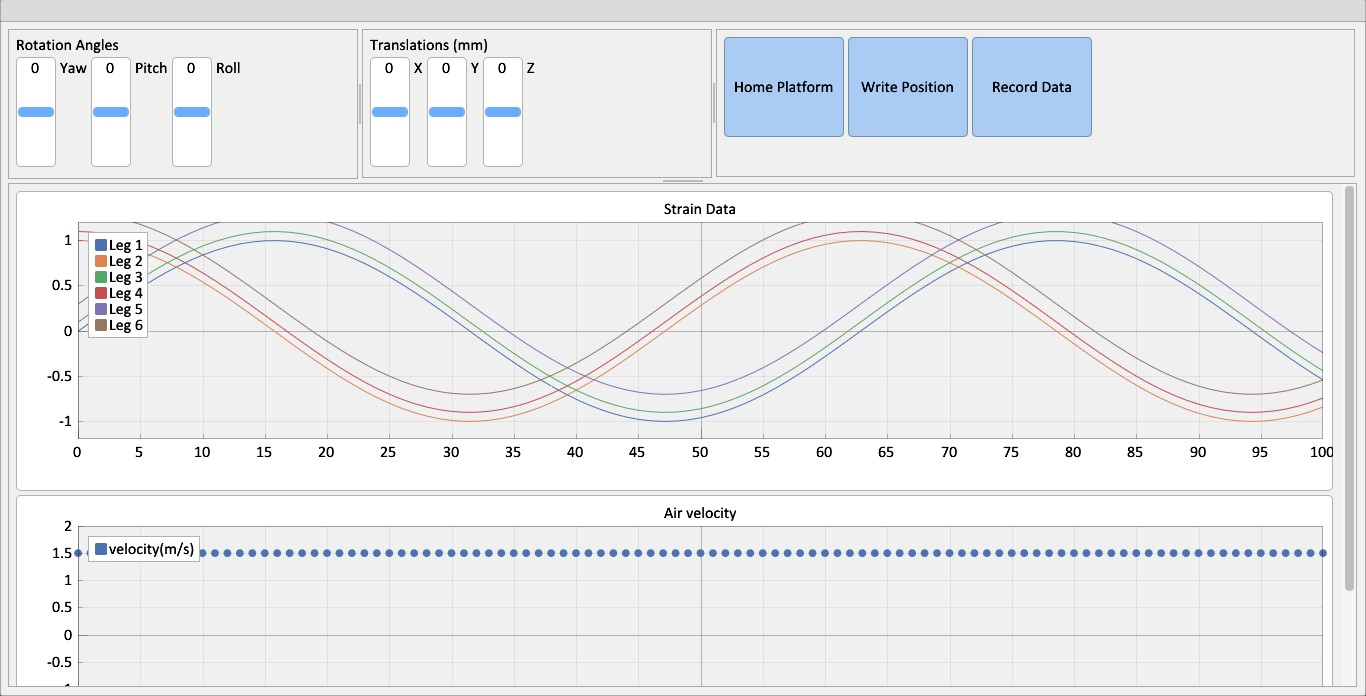
\includegraphics[width=1\linewidth]{Figures/hmi}
	\caption[HMI Dashboard]{HMI Dashboard}
	\end{figure}
\end{center}

This includes slider buttons to control platform position and orientation. It also includes buttons to allow for data capture  and platform control. The dashboard also has a live plot of incoming data to provide immediate user feedback.

\section{PCB}
The schematics from the electrical designs as seen in the appendix were routed to generate a PCB ready for manufacture. This is shown in the 3D render below:
\begin{center}
	\begin{figure}[H]
	\centering
	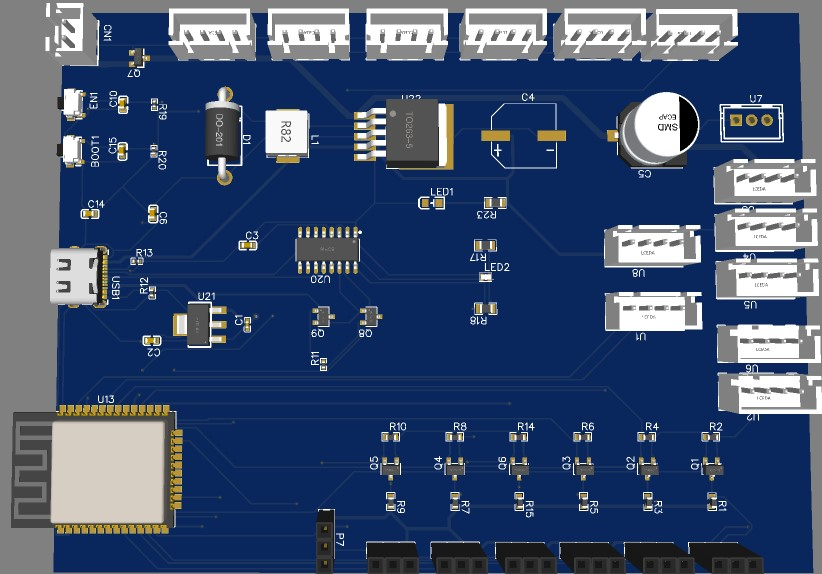
\includegraphics[width=0.7\linewidth]{Figures/pcb}
	\caption[Printed Circuit Board view]{Printed Circuit Board view}
	\end{figure}
\end{center}
